\subsection{Replication}

\subsubsection{Close Replication: Testing prior findings}
\begin{figure}[H]  % 'p' puts it on its own page
    \centering
    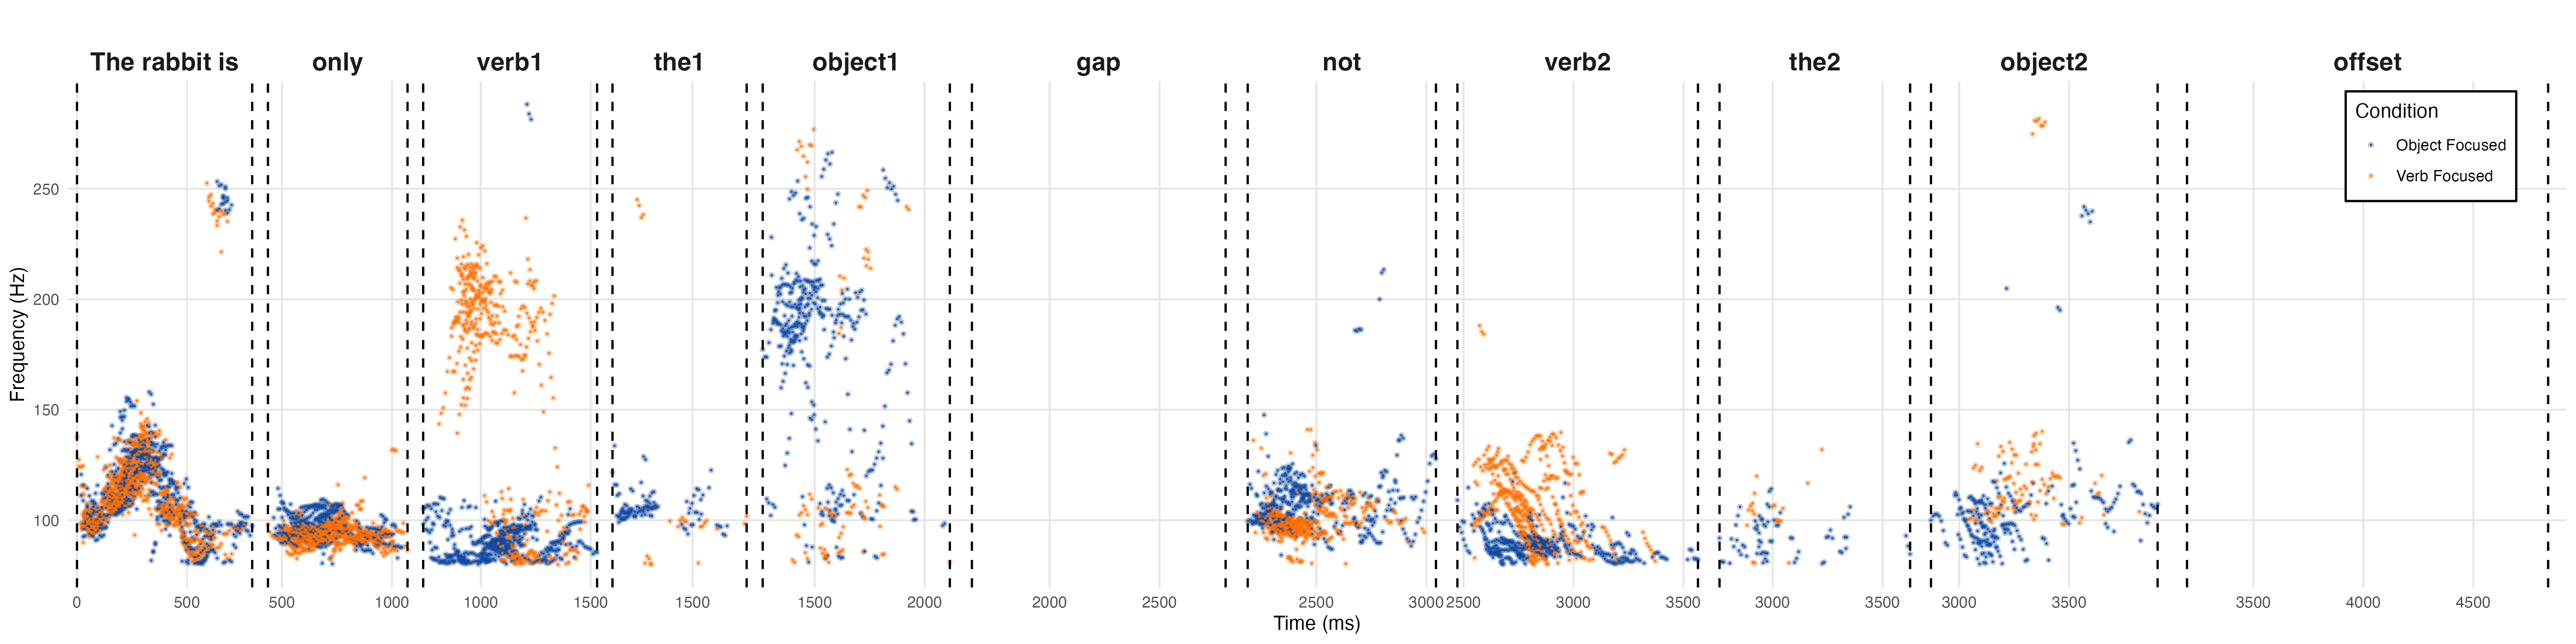
\includegraphics[width=\textwidth,height=\textheight,keepaspectratio]{viz/accoustic.png}
    \caption{things}
    \label{fig:acoustic}
\end{figure}

L1 

\begin{figure}[H]  % 'p' puts it on its own page
    \centering
    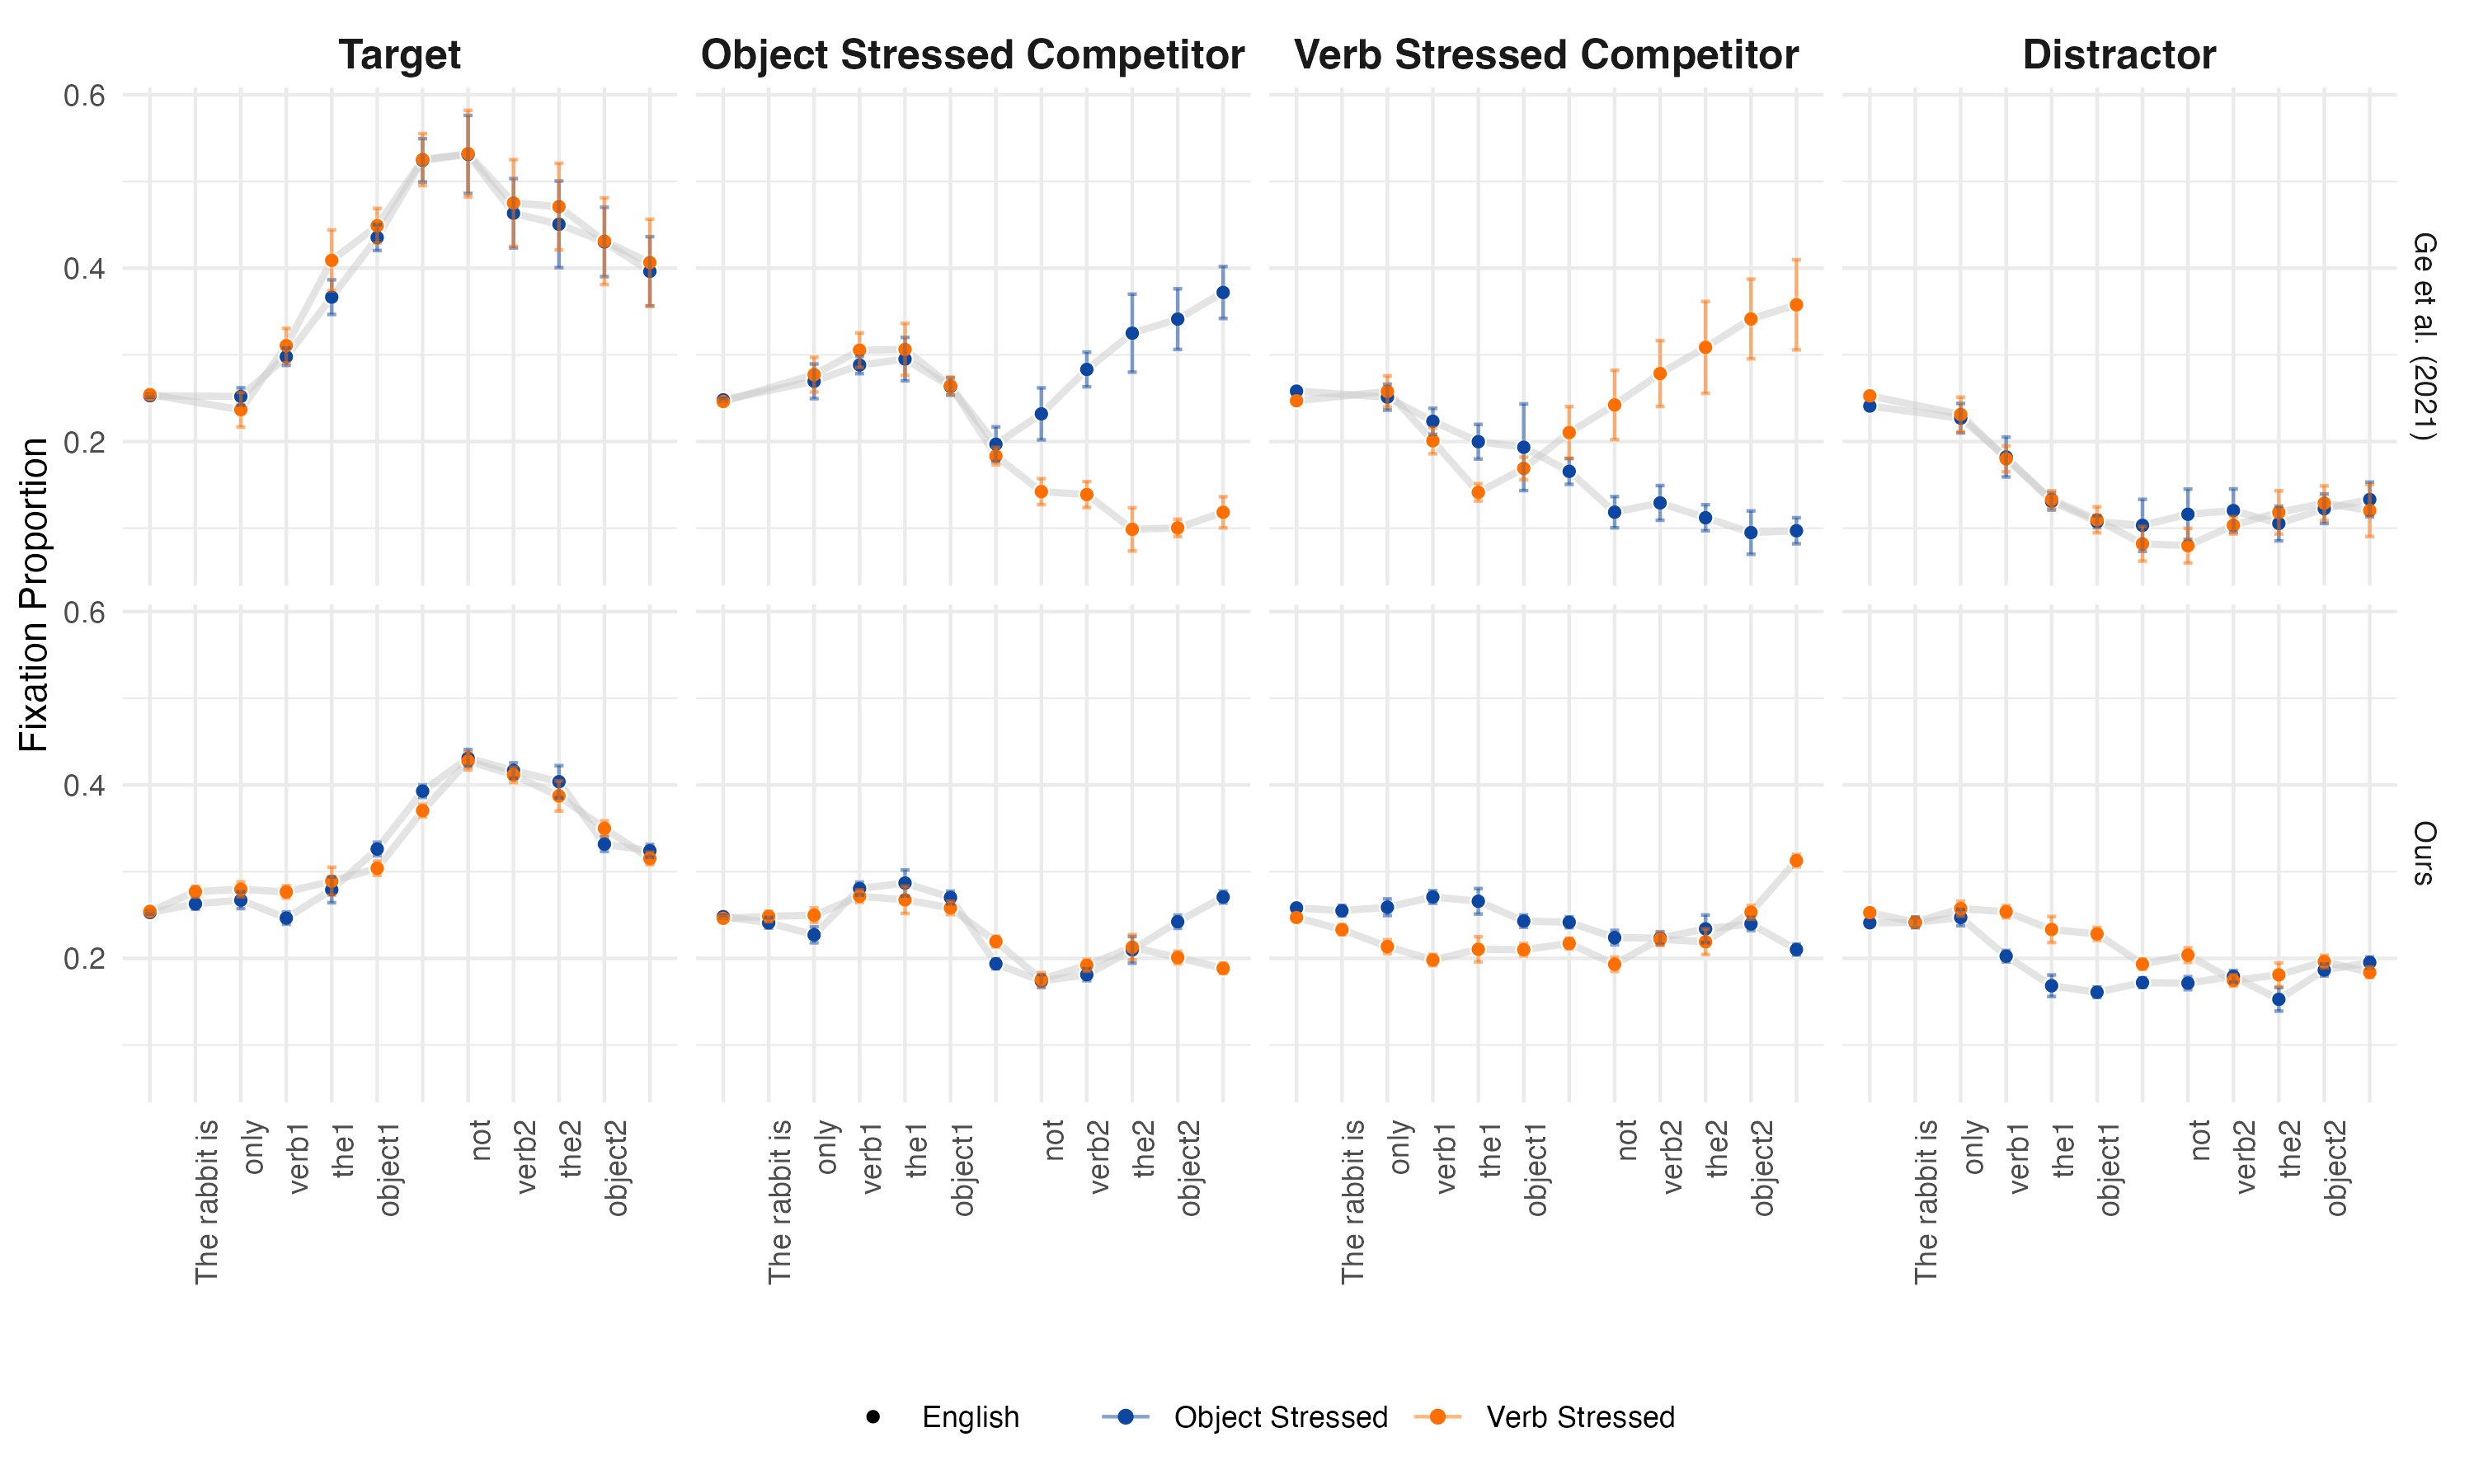
\includegraphics[width=\textwidth,height=\textheight,keepaspectratio]{viz/english_fix.png}
    \caption{things}
    \label{fig:english_fix}
\end{figure}

\begin{figure}[H]  % 'p' puts it on its own page
    \centering
    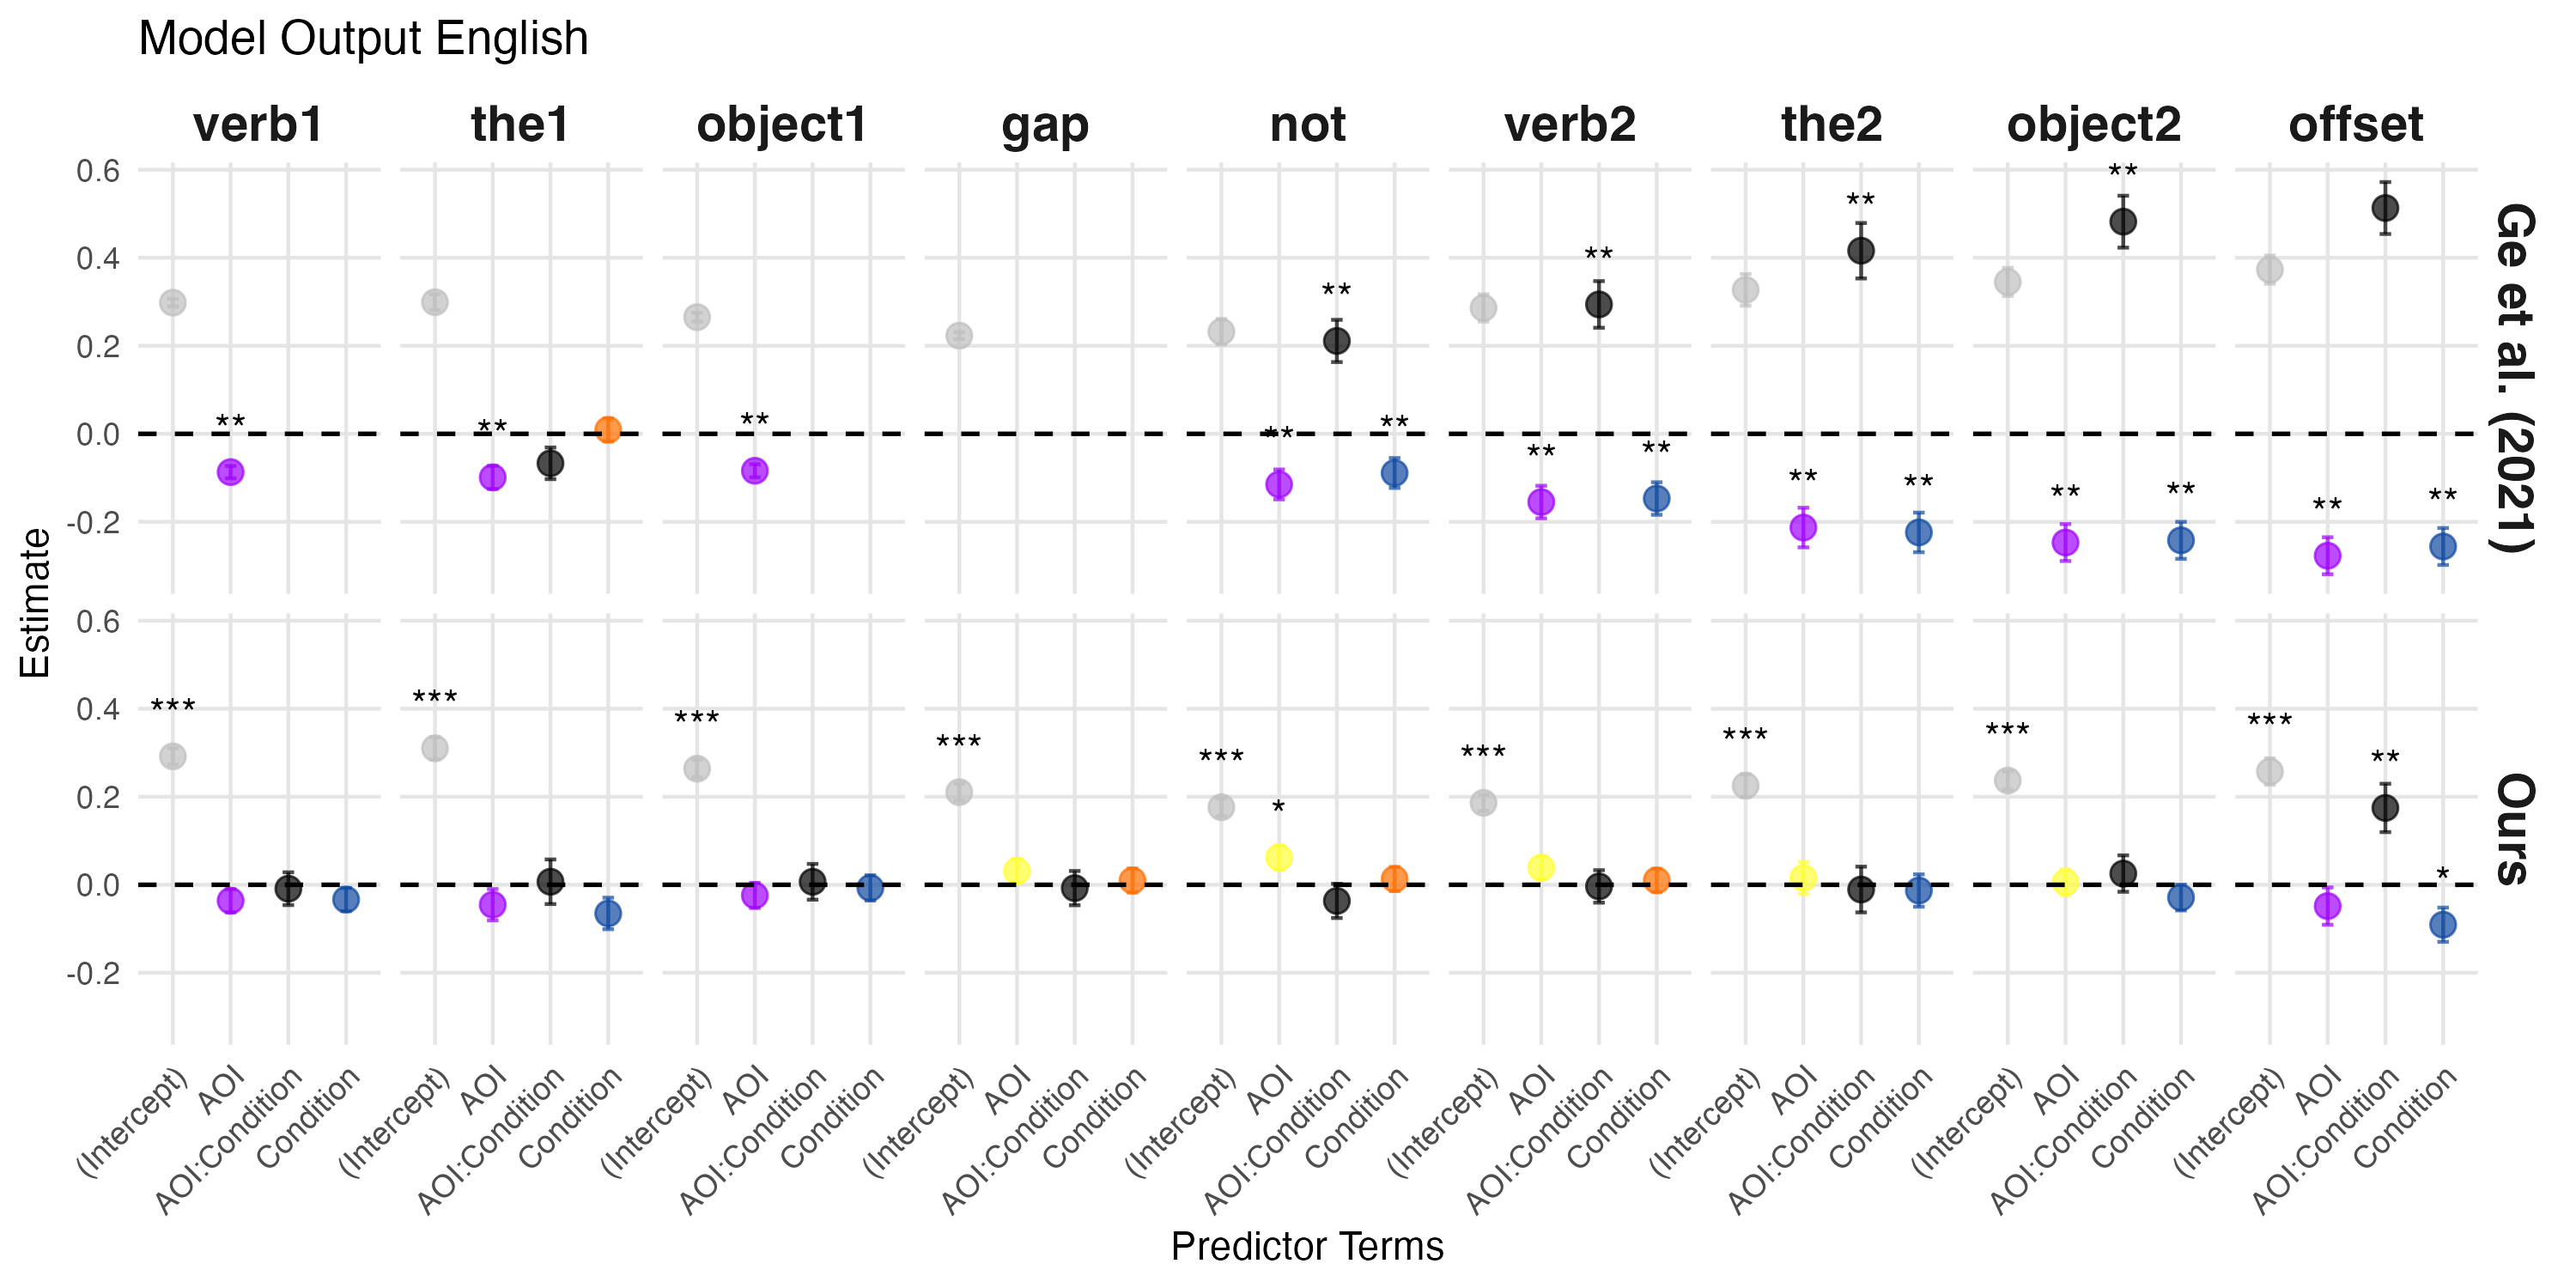
\includegraphics[width=\textwidth,height=\textheight,keepaspectratio]{viz/model_plot_english.png}
    \caption{things}
    \label{fig:model_plot_english}
\end{figure}

L2

\begin{figure}[H]  % 'p' puts it on its own page
    \centering
    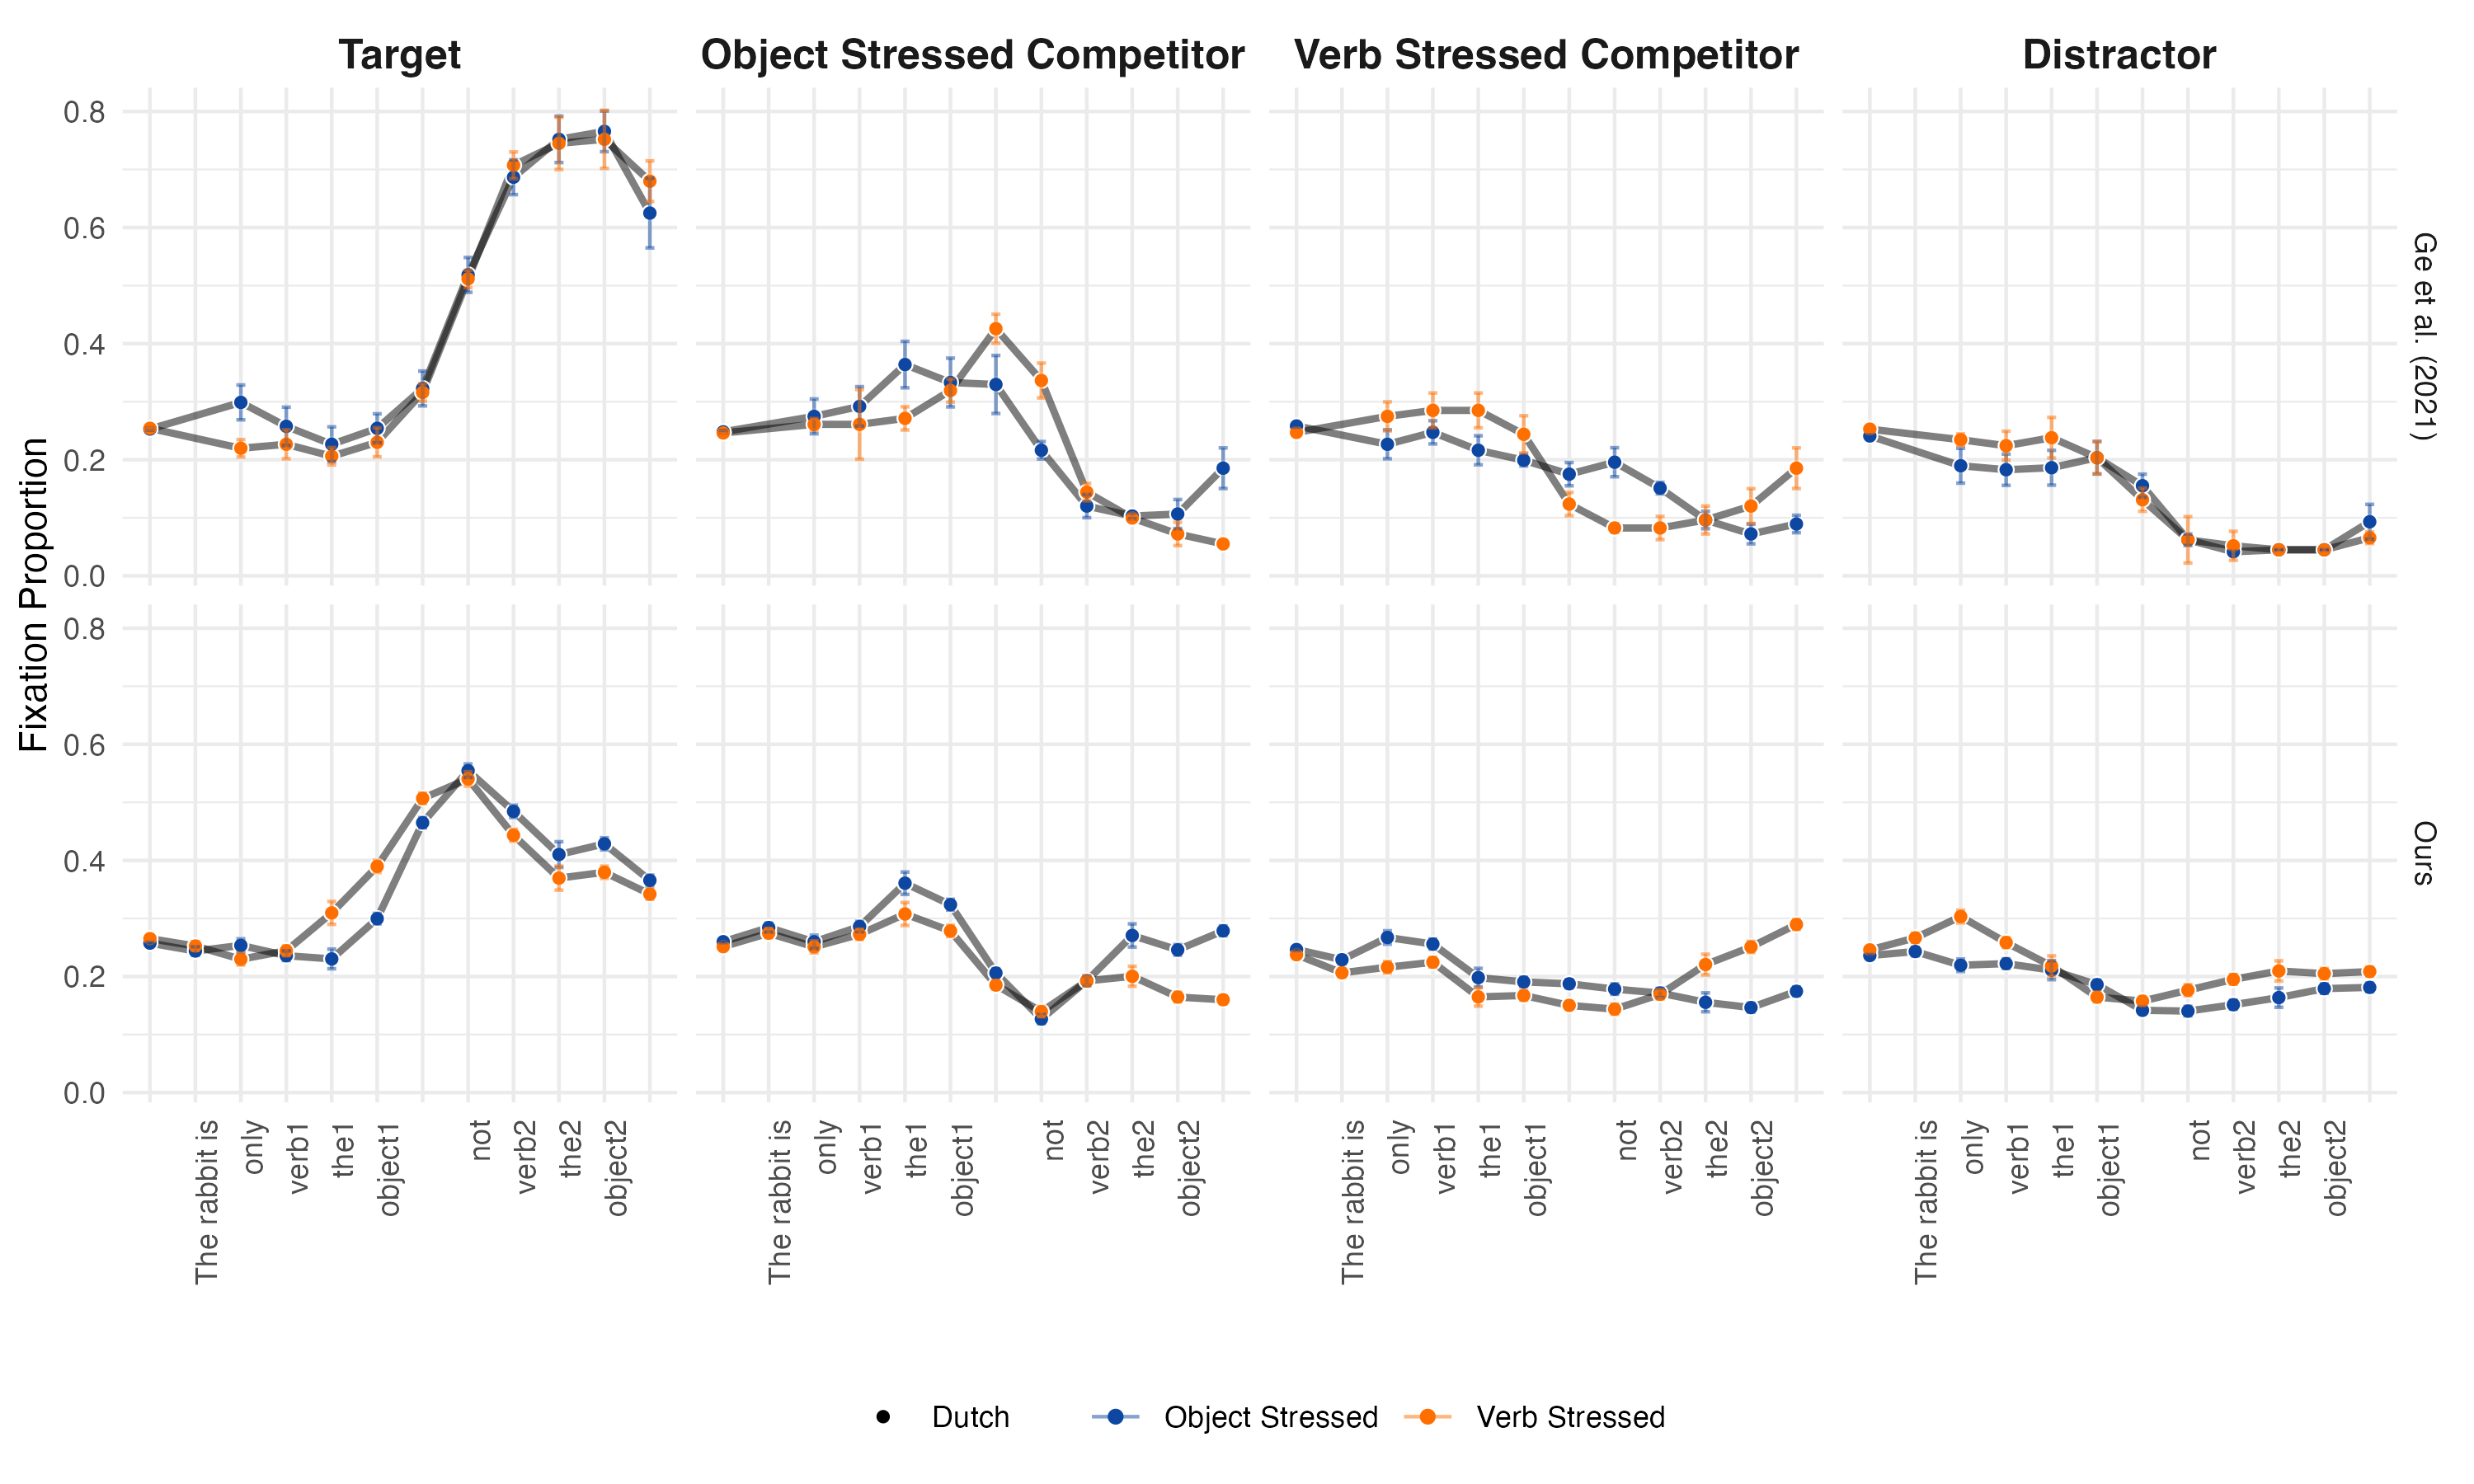
\includegraphics[width=\textwidth,height=\textheight,keepaspectratio]{viz/dutch_fix.png}
    \caption{things}
    \label{fig:dutch_fix}
\end{figure}


\begin{figure}[H]  % 'p' puts it on its own page
    \centering
    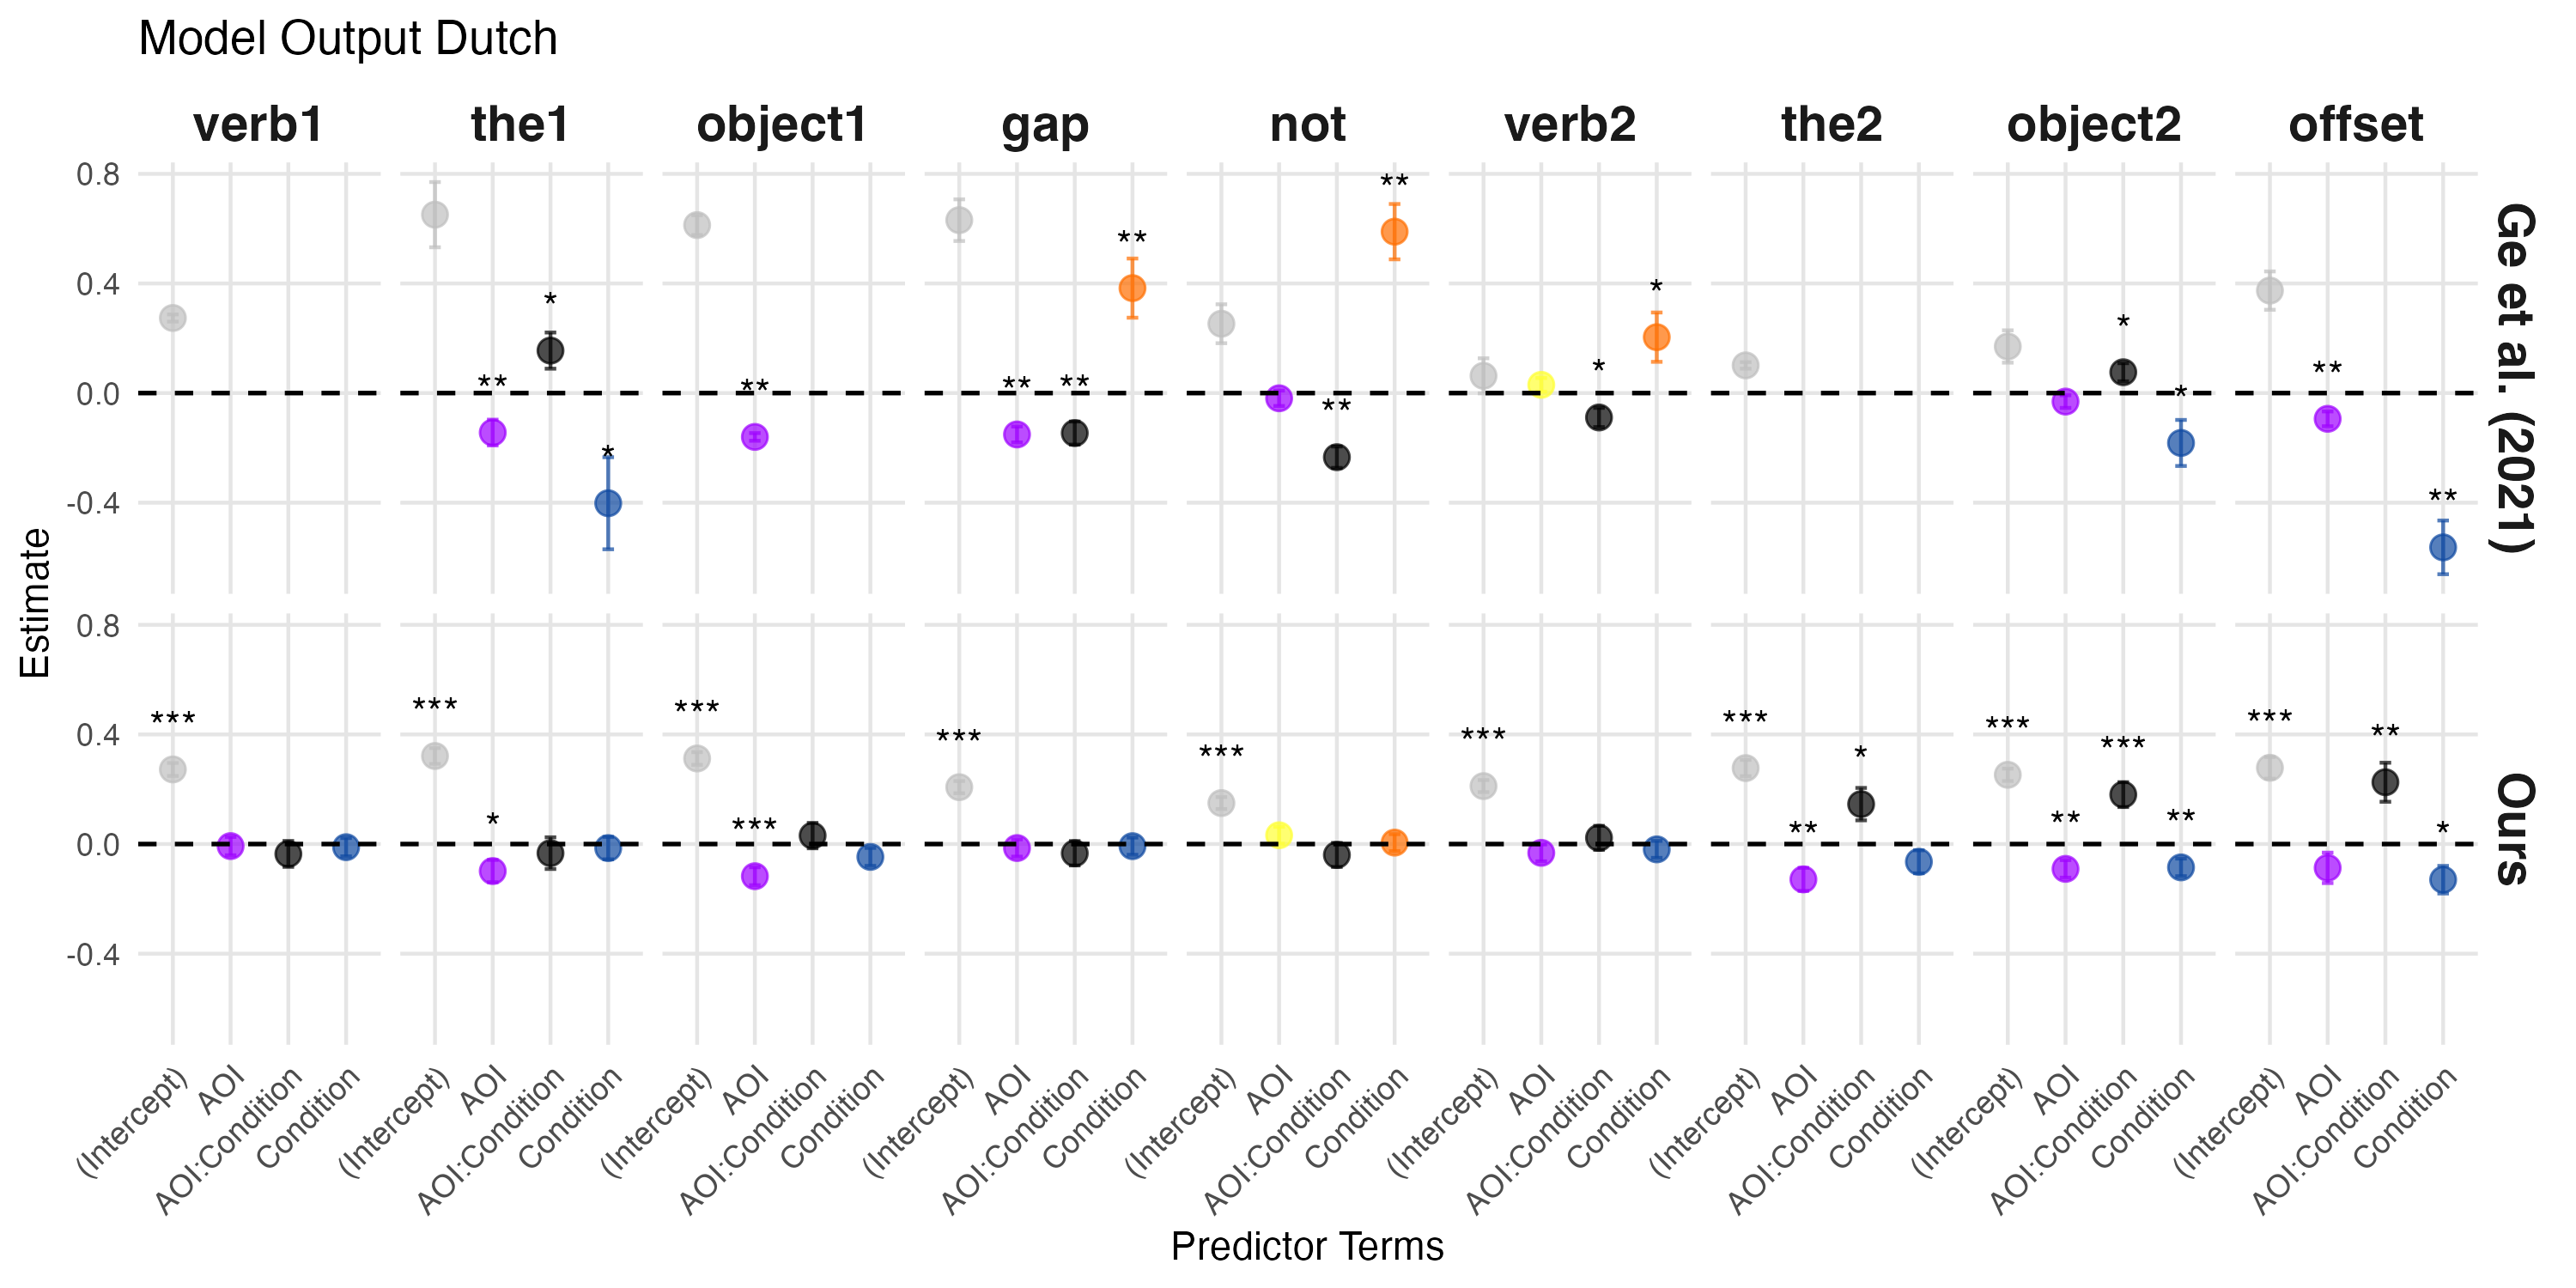
\includegraphics[width=\textwidth,height=\textheight,keepaspectratio]{viz/model_plot_dutch.png}
    \caption{things}
    \label{fig:model_plot_dutch}
\end{figure}


\subsubsection{Methodological refinement: A "focused" approach}



L1 

\begin{figure}[H]  % 'p' puts it on its own page
    \centering
    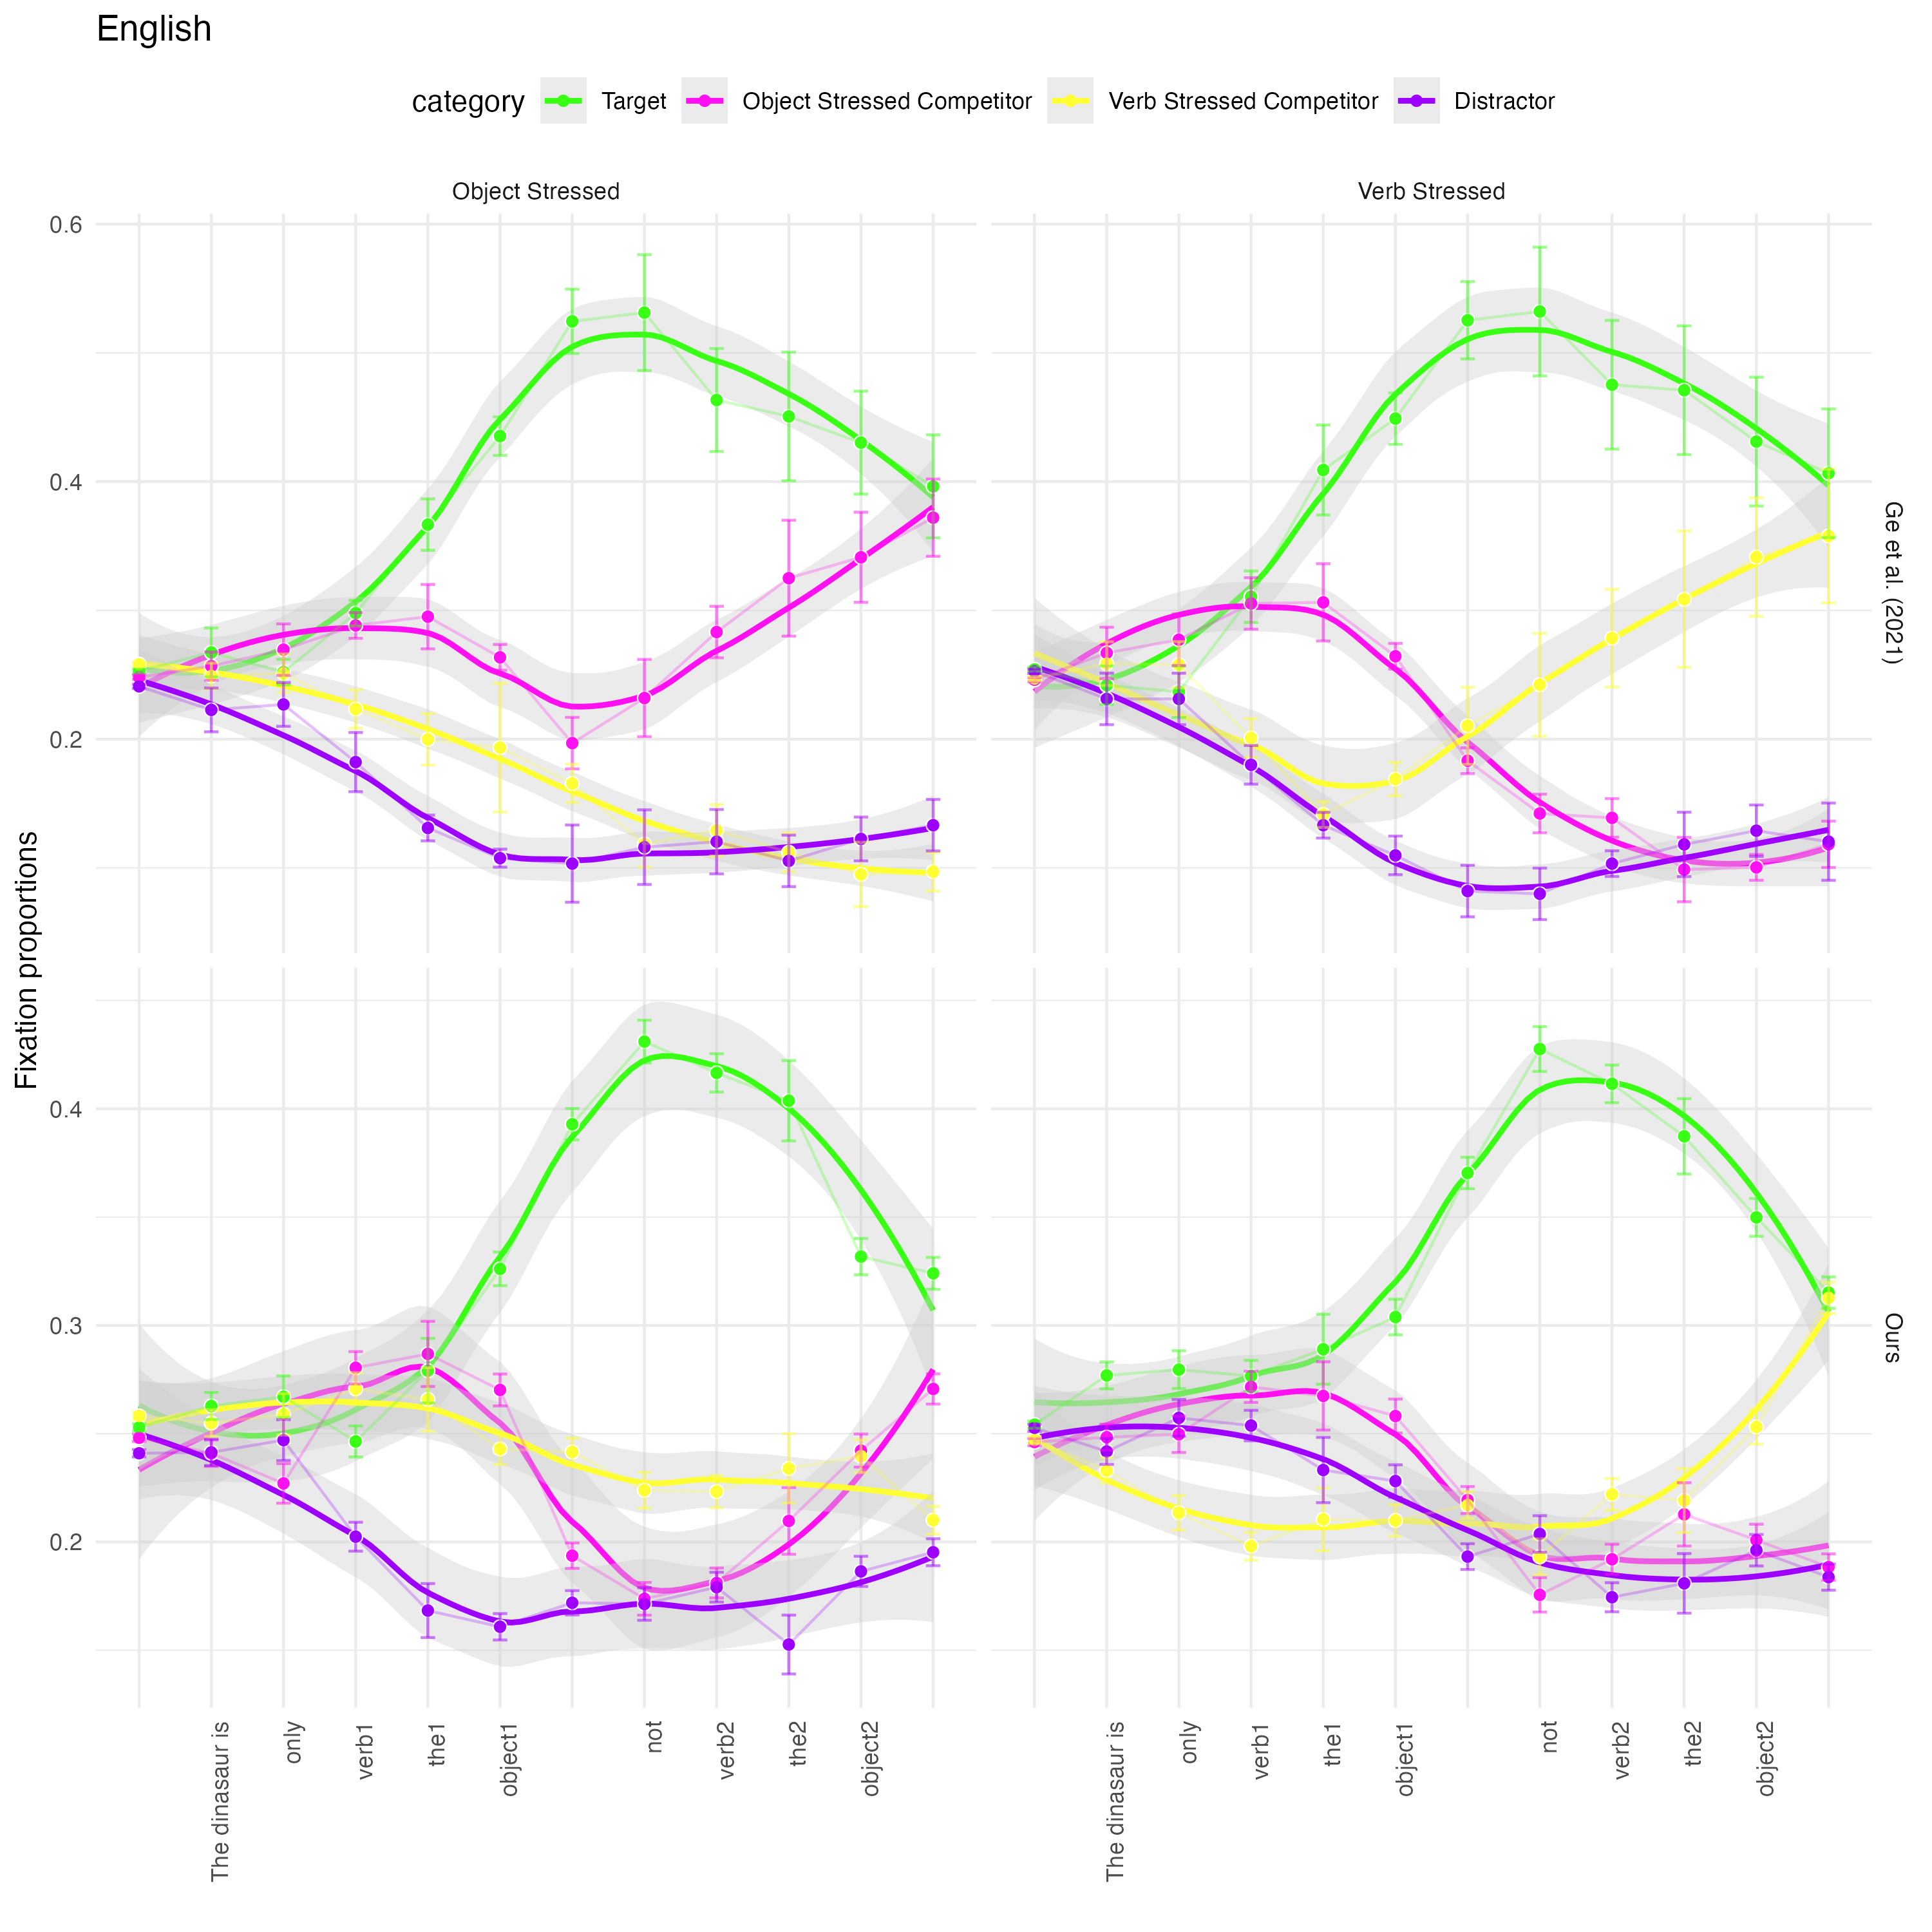
\includegraphics[width=\textwidth,height=\textheight,keepaspectratio]{viz/english_fix2.png}
    \caption{things}
    \label{fig:english_fix2}
\end{figure}

L2

\begin{figure}[H]  % 'p' puts it on its own page
    \centering
    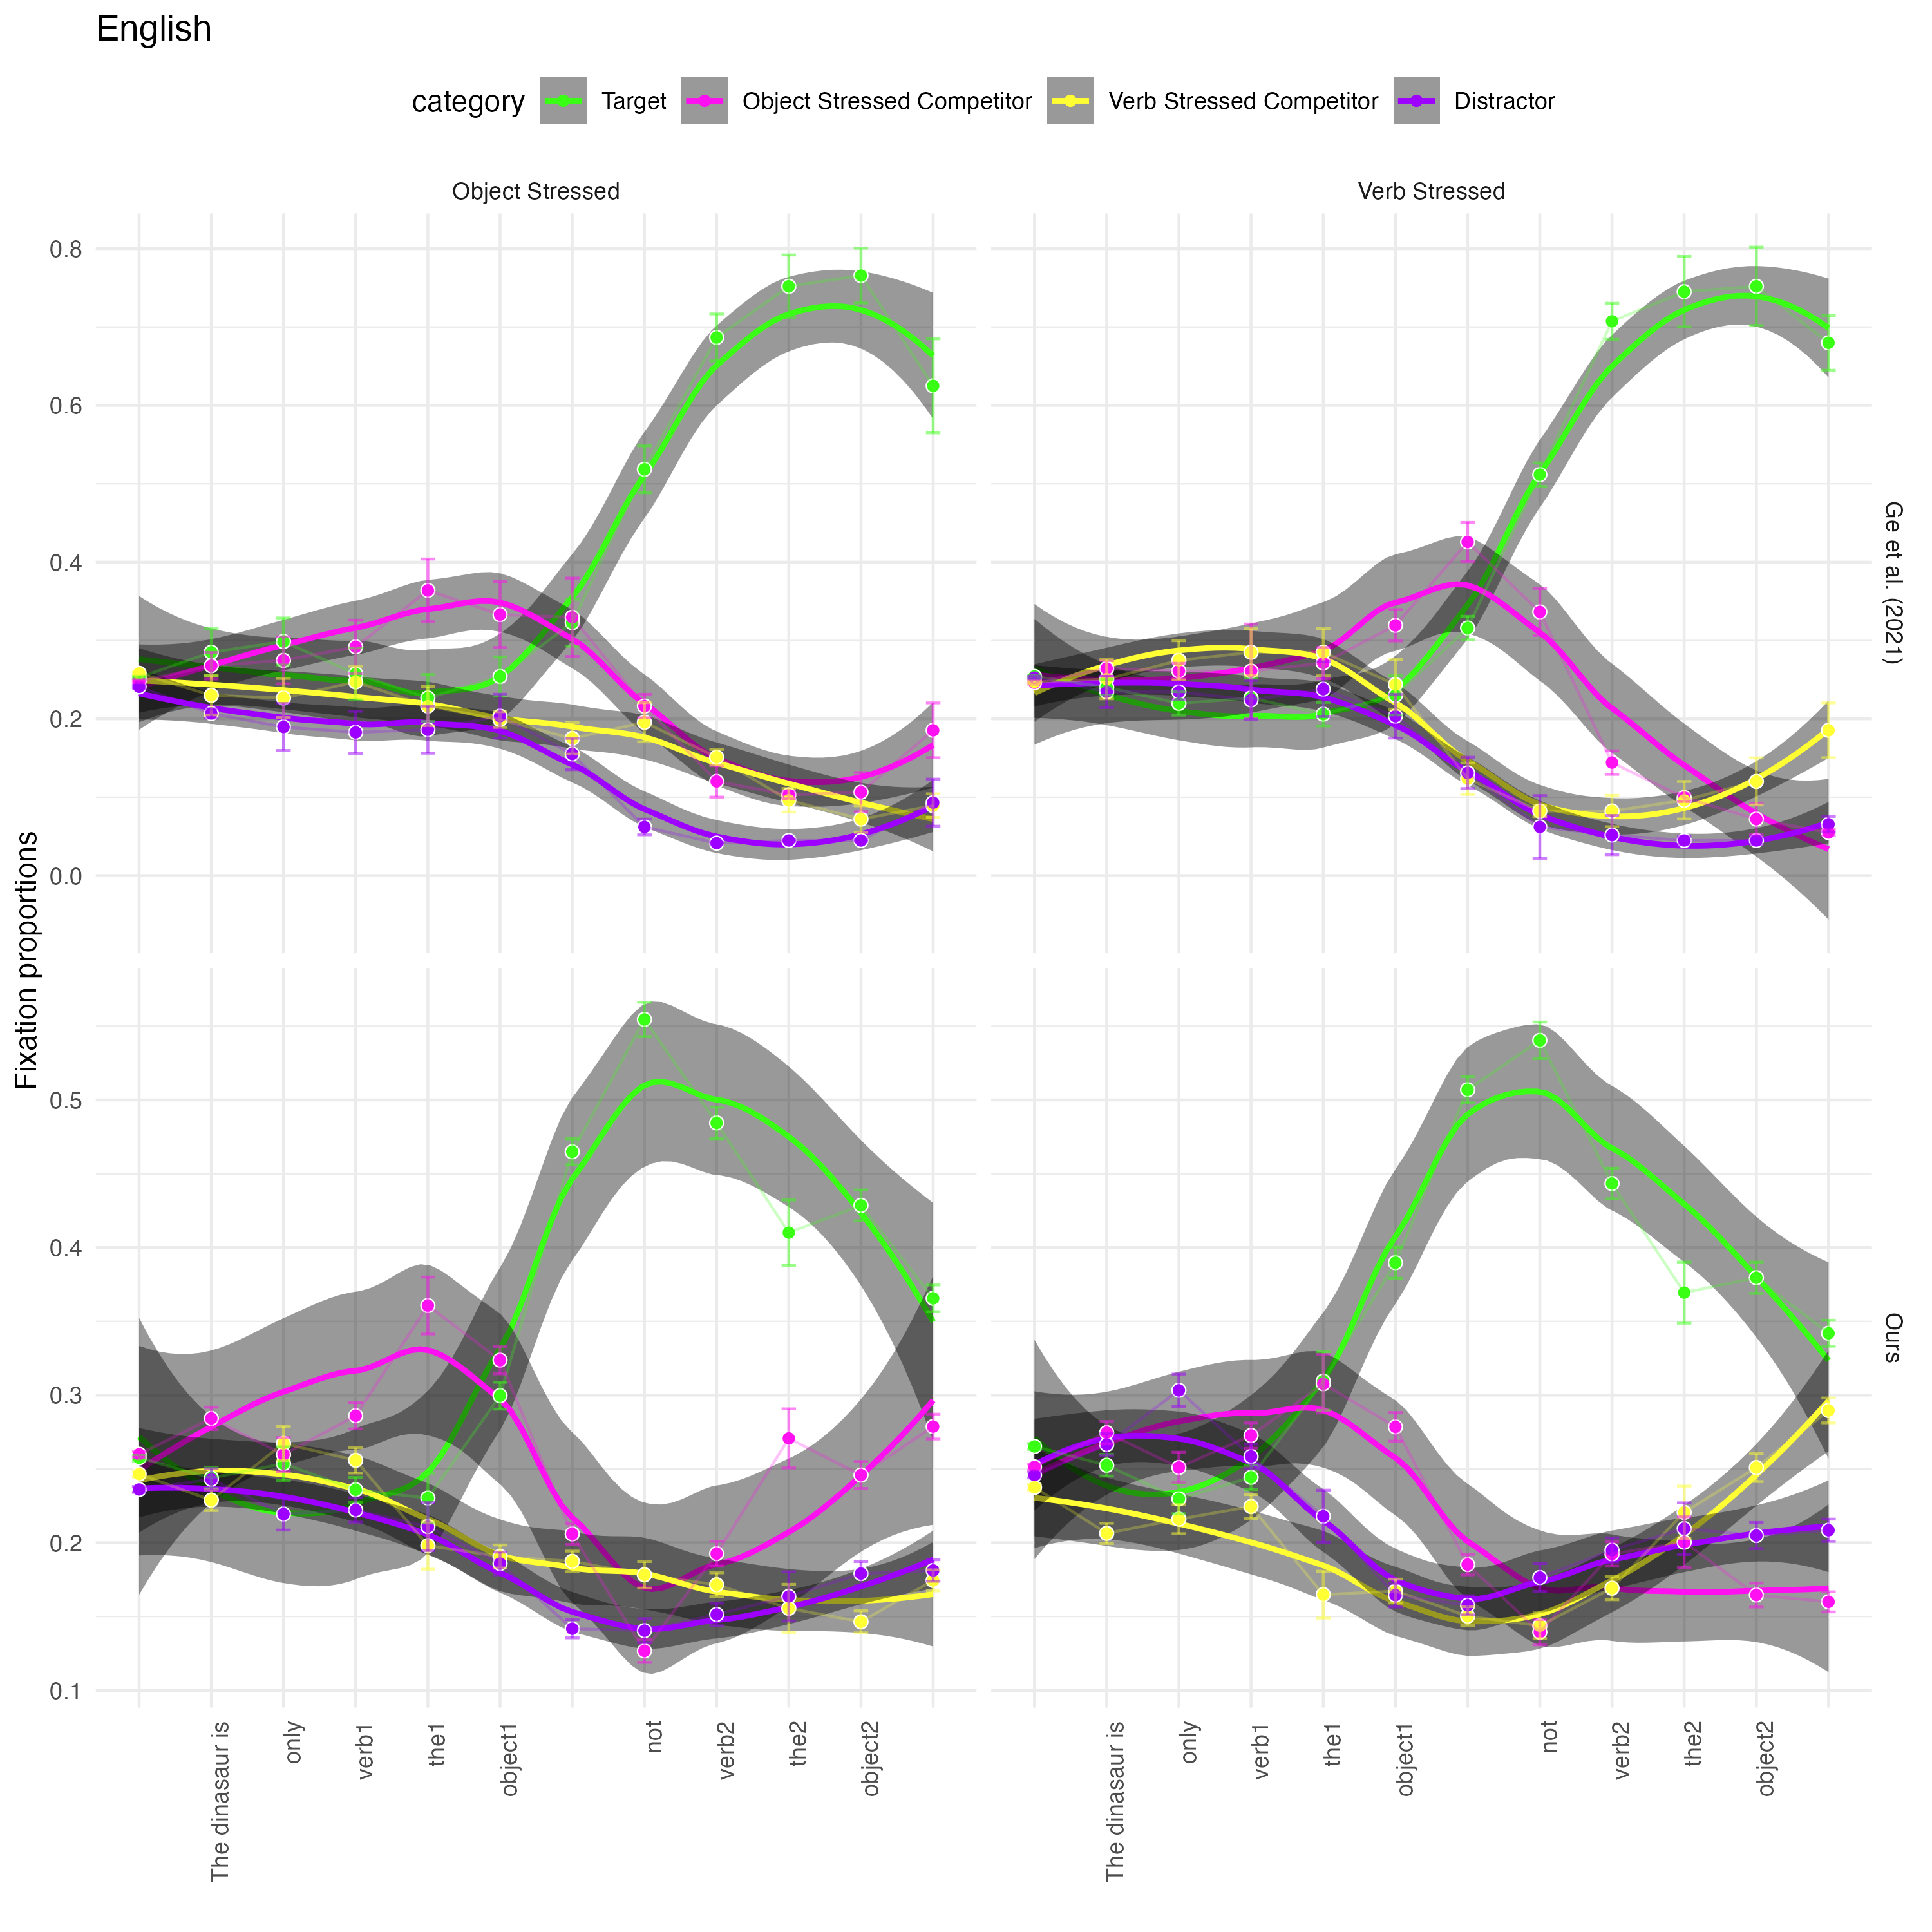
\includegraphics[width=\textwidth,height=\textheight,keepaspectratio]{viz/dutch_fix2.png}
    \caption{things}
    \label{fig:english_fix2}
\end{figure}

\begin{figure}[H]  % 'p' puts it on its own page
    \centering
    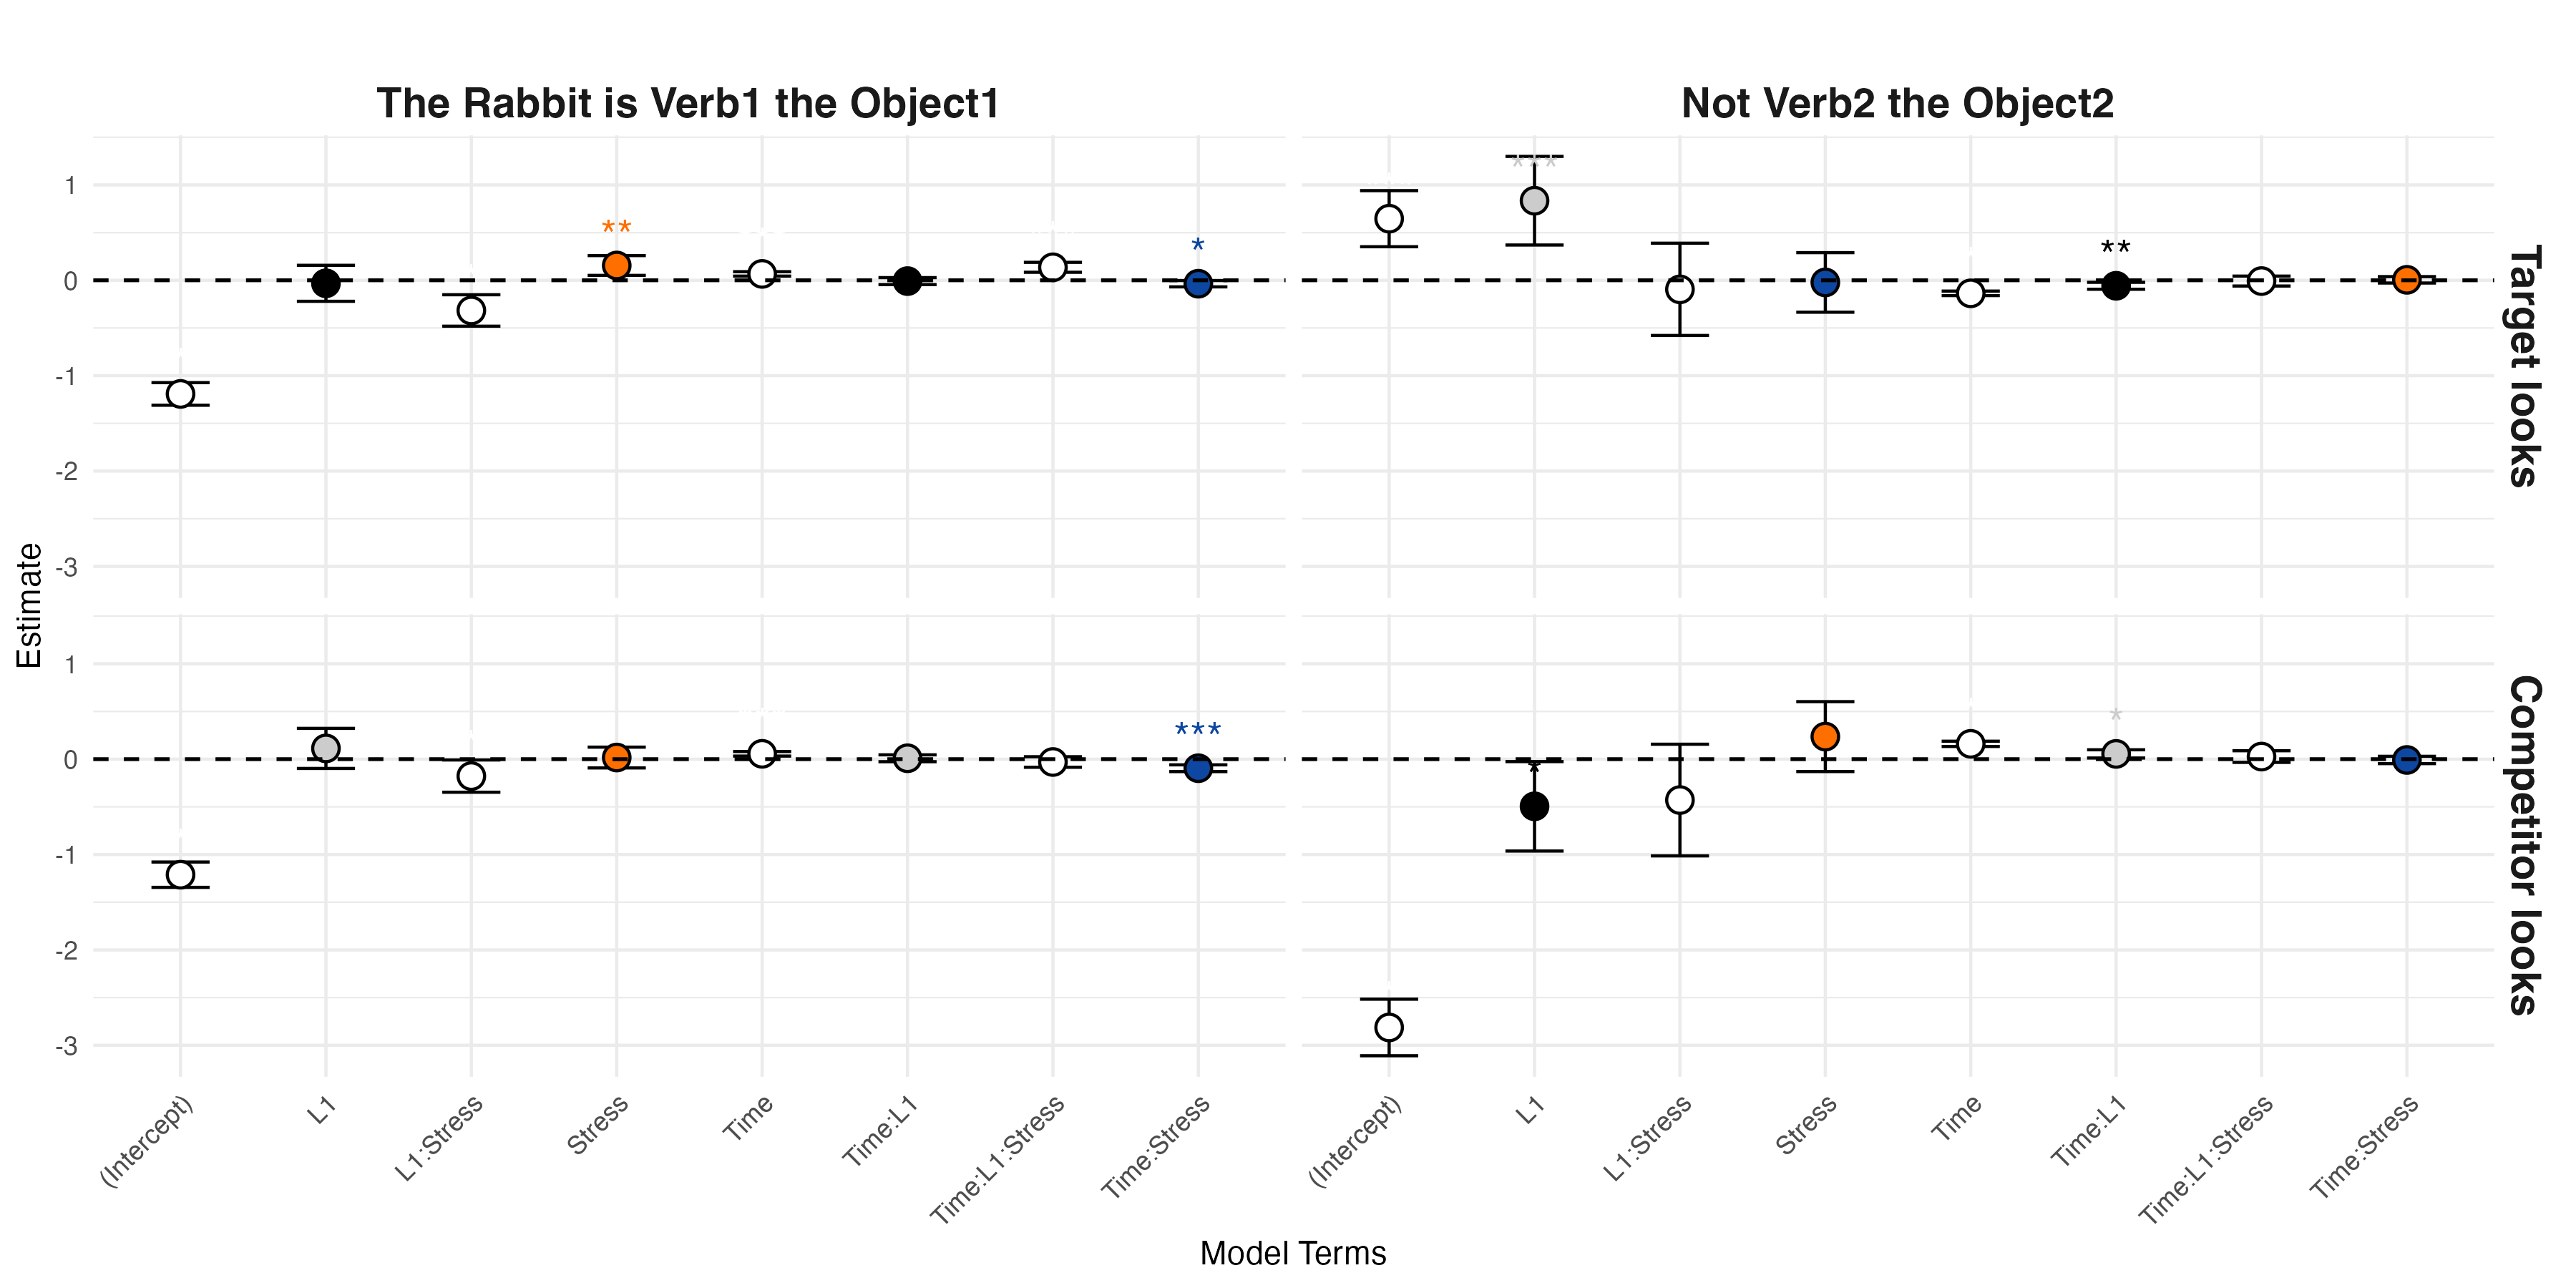
\includegraphics[width=\textwidth,height=\textheight,keepaspectratio]{viz/gam_mod_out.png}
    \caption{things}
    \label{fig:gam_mod_out}
\end{figure}

\subsection{Extension}

Individual difference plot:
\clearpage
\begin{figure}[p]  % 'p' puts it on its own page
    \centering
    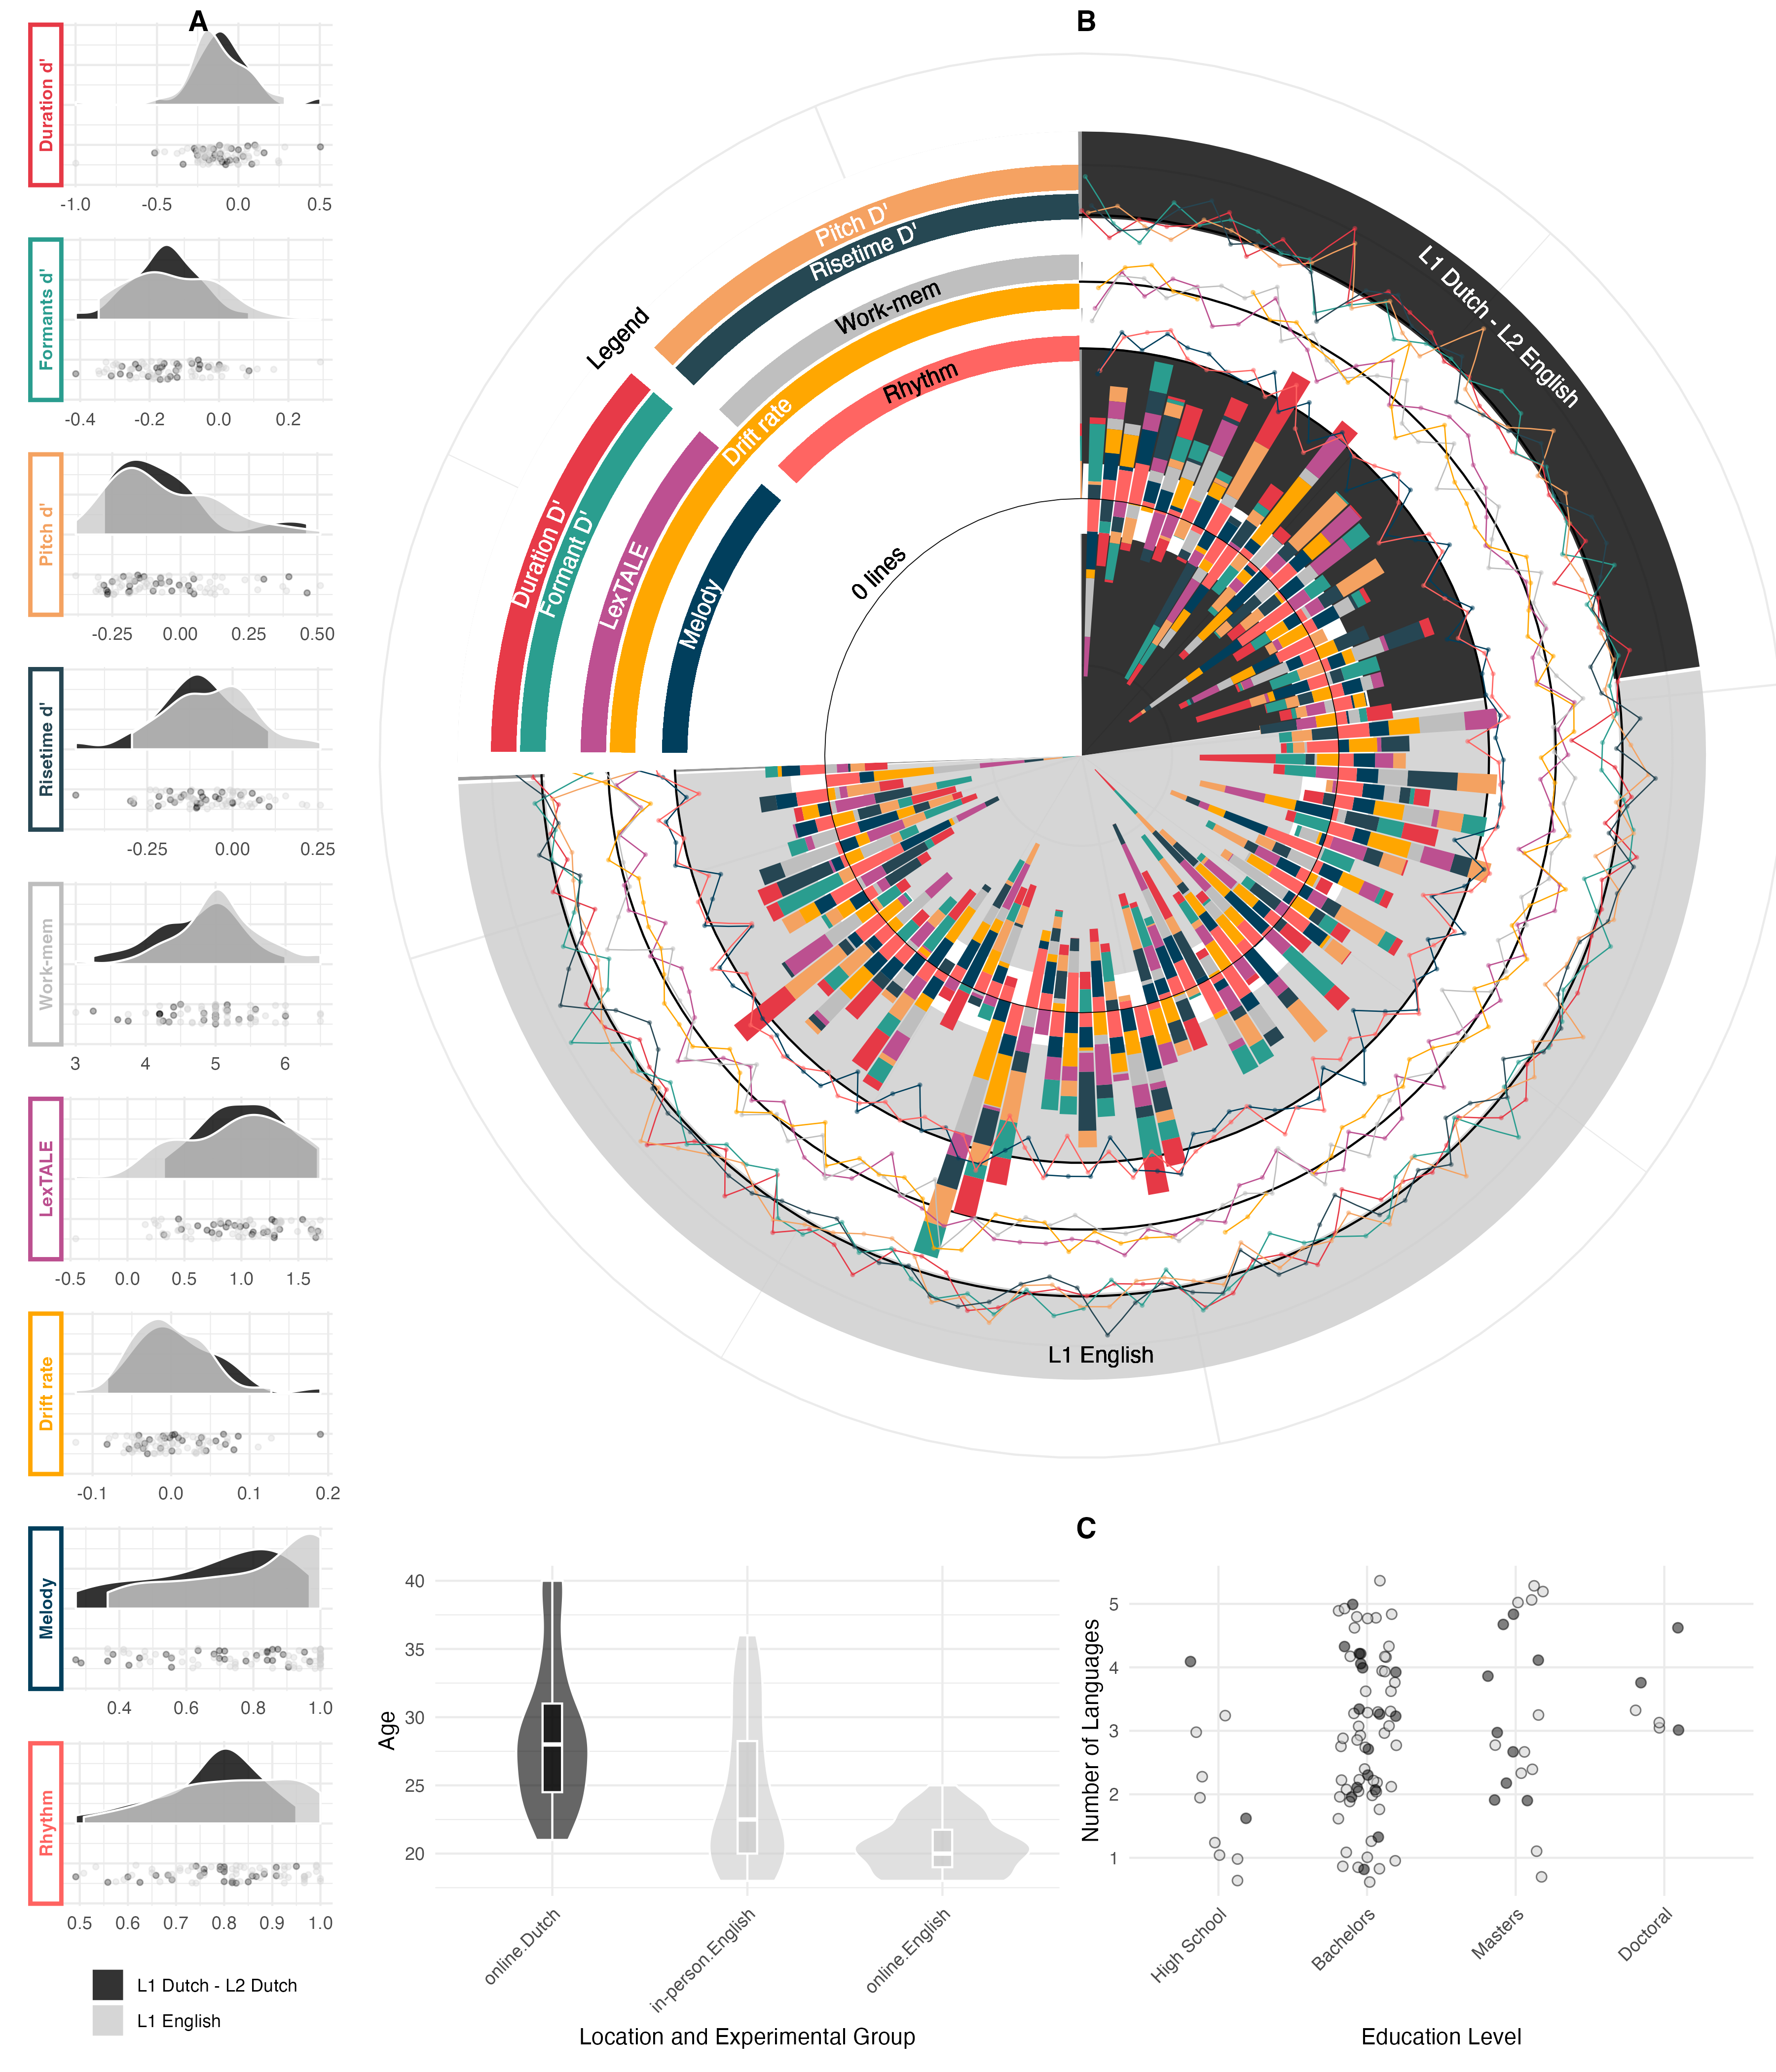
\includegraphics[width=\textwidth,height=\textheight,keepaspectratio]{viz/combined_plot_circle.png}
    \caption{describe what is going on here- A- tasks across the Dutch and English, B individual difference vectors for each participant, C background information on participants}
    \label{fig:combined_plot}
\end{figure}
\clearpage

\begin{figure}[H]  % 'p' puts it on its own page
    \centering
    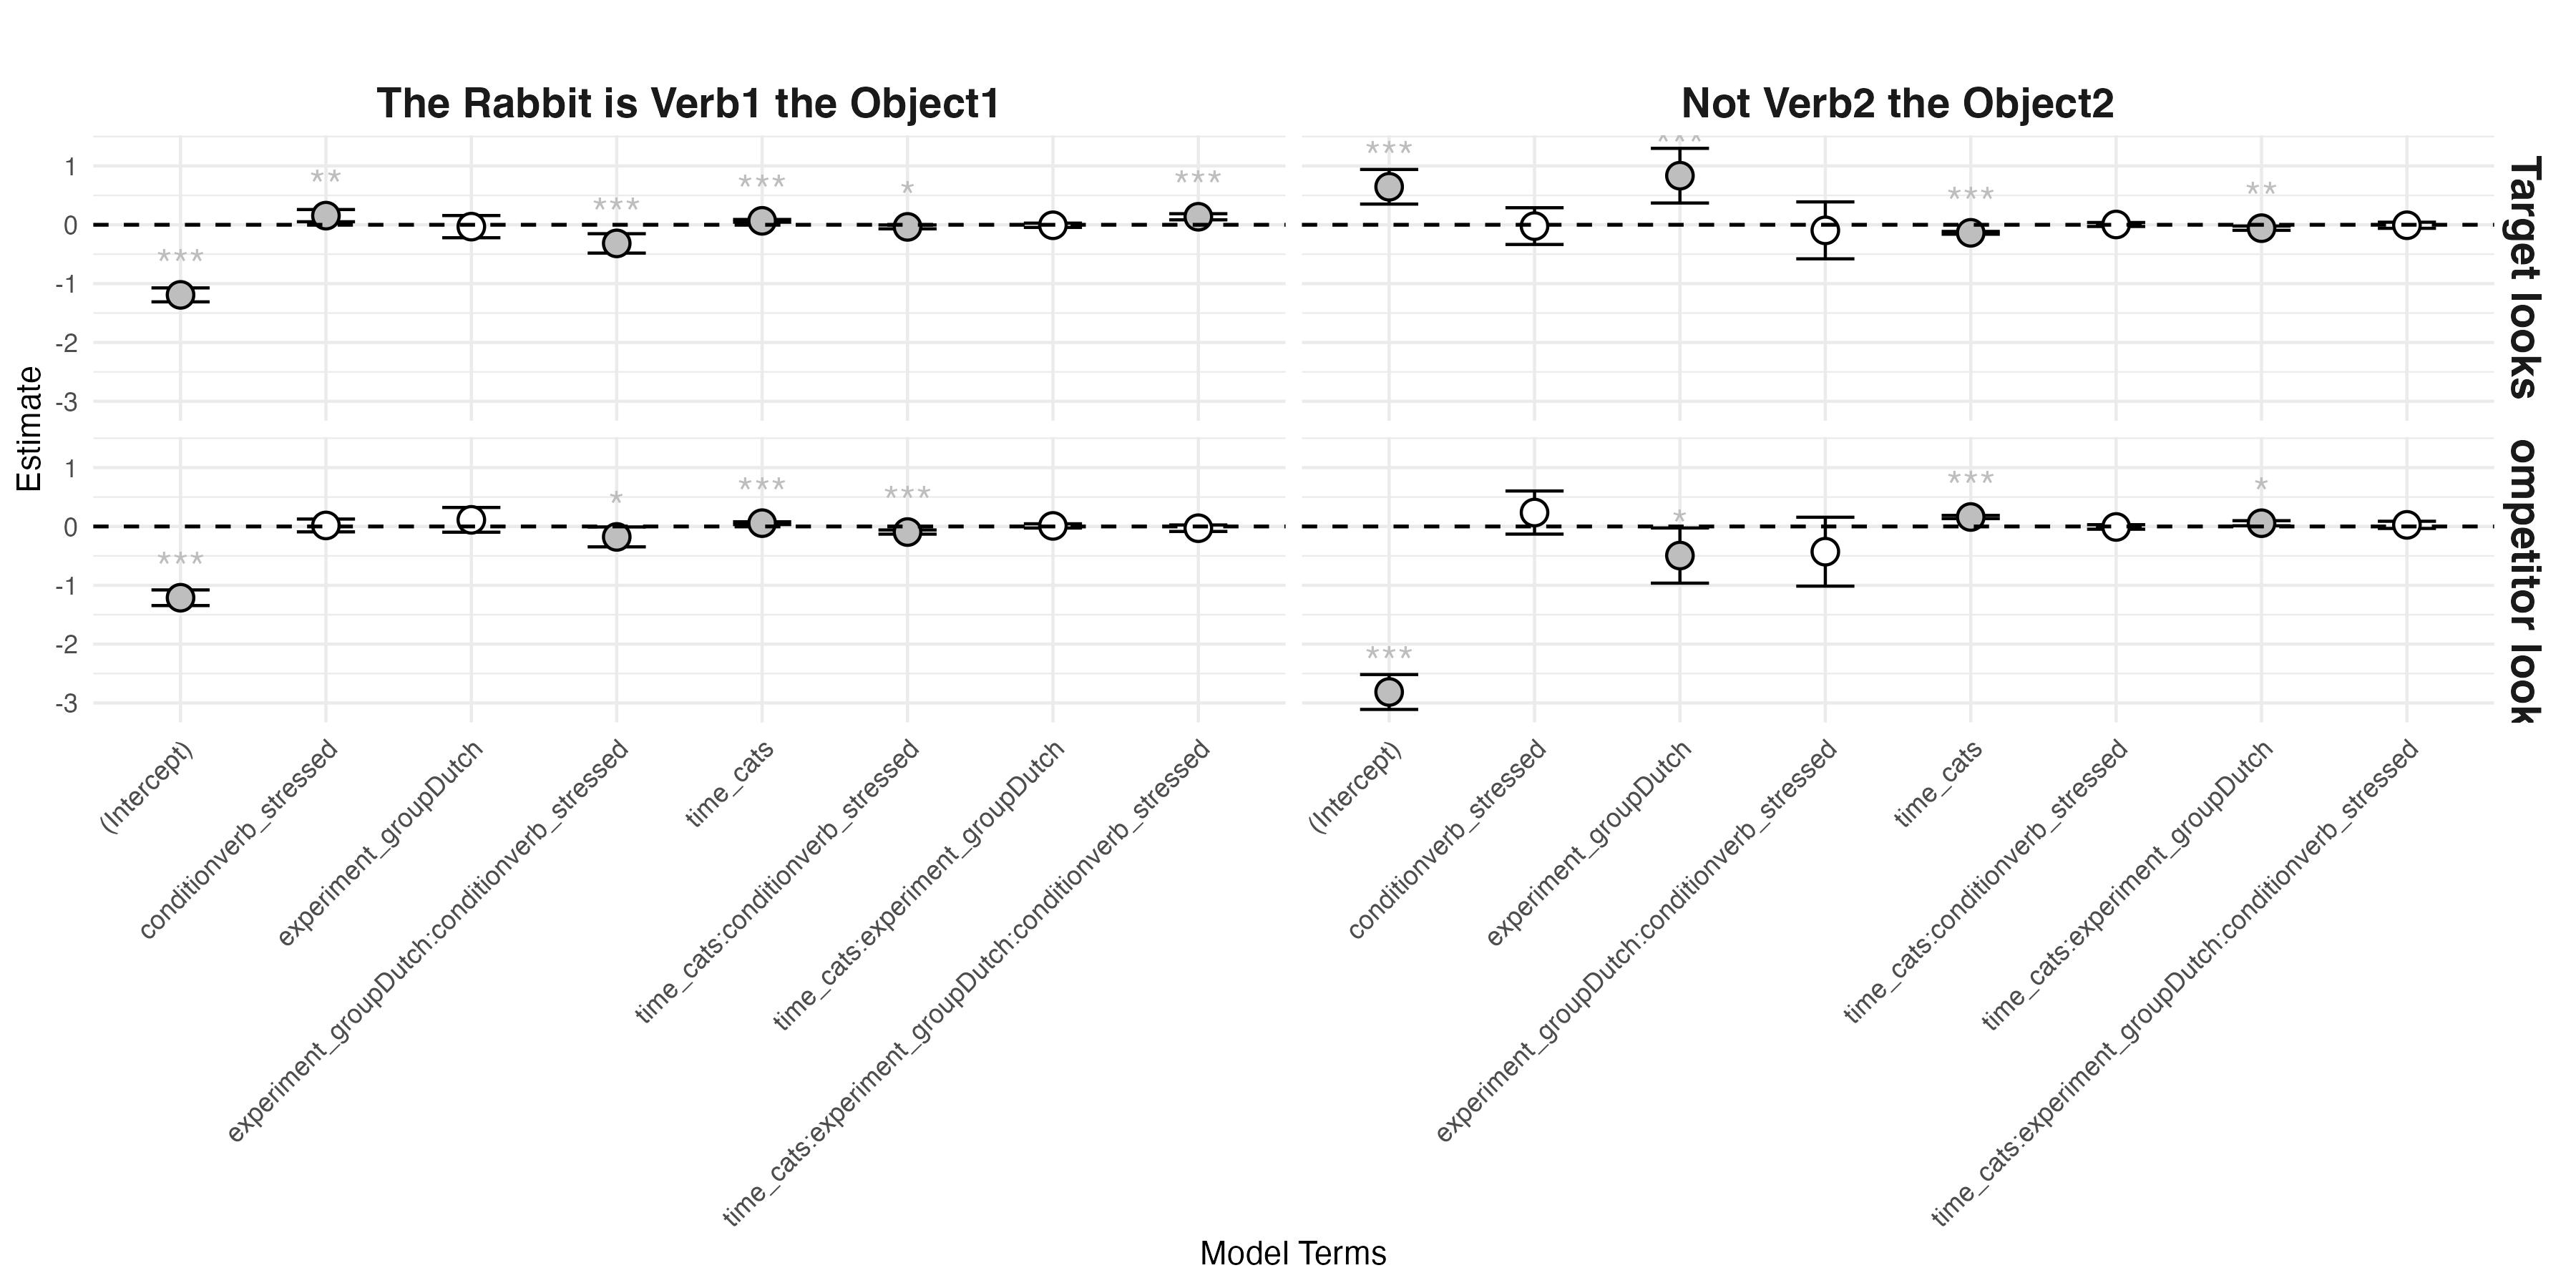
\includegraphics[width=\textwidth,height=\textheight,keepaspectratio]{viz/id_gam_mod_out.png}
    \caption{describe what is going on here- colorized by individual difference measure. Only significant variables are colored (white indicates non-significance). Grey indicates significant but not and individual difference measure}
    \label{fig:id_gam_mod_out}
\end{figure}

L1 

L2


